\documentclass[varwidth=true, border=2pt]{standalone}
\usepackage{tkz-euclide}

\begin{document}
\usetkzobj{all}
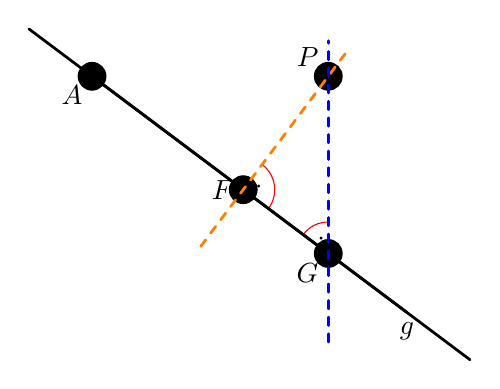
\begin{tikzpicture}
    \tkzSetUpPoint[shape=circle,size=10,color=black,fill=black]
    \tkzSetUpLine[line width=1]
    \tkzDefPoints{0/3/A, 4/0/B, 3/3/P, 3/0.75/G}
    \tkzDefLine[perpendicular=through P,/tikz/overlay](A,B)\tkzGetPoint{x}
    \tkzInterLL(A,B)(P,x) \tkzGetPoint{F}

    \tkzMarkAngle[arc=l,size=0.4cm,color=red,fill=red!20](B,F,P)
    \tkzLabelAngle[pos = 0.2](B,F,P){$\cdot$}

    \tkzMarkAngle[arc=l,size=0.4cm,color=red,fill=red!20](P,G,A)
    \tkzLabelAngle[pos = 0.2](P,G,A){$\cdot$}

    \tkzDrawPoints(A,F,P,G)


    \tkzDrawSegments(A,B)
    \tkzDrawLines(A,B)
    \tkzDrawLine[dashed,color=orange,add=0.5 and 0.2](F,P)
    \tkzDrawLine[dashed,color=blue,add=0.5 and 0.2](G,P)
    %
    \tkzLabelPoint[below left](A){$A$}
    \tkzLabelPoint[below left](G){$G$}
    \tkzLabelPoint[above left](P){$P$}
    \tkzLabelPoint[left](F){$F$}
    \tkzLabelLine[below,pos=1](A,B){$g$}
\end{tikzpicture}
\end{document}
